\documentclass{beamer}

\setbeamertemplate{navigation symbols}{} % don't use navigation tools on slides

\usepackage[absolute,overlay]{textpos}
\usepackage{extrabeamercmds}
    
    
\begin{document}

\frame{
    \frametitle{Example}
    
    An example full frame video using \textbf{commands from extrabeamercmds} is on the next slide.
}


\fullFrameMovie[loop]{apollo17.avi}{apollo17.jpg}{\CopyrightText{Apollo 17, NASA}}
    
\frame{
    \frametitle{Example 2}
    
    An example full frame video using the \textbf{basic syntax} is on this slide.
    
    \vspace{20pt}
    
    \href{run:apollo17.avi?autostart&loop}{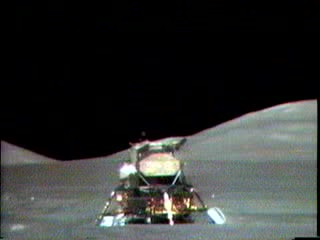
\includegraphics[height=0.7\textheight]{apollo17.jpg}}
}


\frame{
    \frametitle{Example 3}
    
    An example full frame video using \textbf{commands from extrabeamercmds} is on the next slide.
}

% this assumes you have a .jpg named the same thing as your .avi
\fullFrameMovieAvi[noloop]{apollo17}{\CopyrightText{Apollo 17, NASA}}

    
\end{document}


